\documentclass{article} % For LaTeX2e
\usepackage{nips12submit_e,times}
%\documentstyle[nips12submit_09,times,art10]{article} % For LaTeX 2.09

\renewcommand{\vec}[1]{\mathbf{#1}} % Bold vectors
\def\argmax{\operatornamewithlimits{arg\max}}

\title{Symbolic Dynamic Programming for Continuous State and Observation POMDPs}


\author
{
Zahra Zamani\\ %\& Scott Sanner\\
ANU \& NICTA\\
Canberra, Australia\\
{\small \texttt{zahra.zamani@anu.edu.au}}\\
%{\small \texttt{first.last@anu.edu.au}}\\
\And
Scott Sanner\\
NICTA \& ANU\\
Canberra, Australia\\
{\small \texttt{scott.sanner@nicta.com.au}}\\
\AND
Pascal Poupart\\
U. of Waterloo\\
Waterloo, Canada\\
{\small \texttt{ppoupart@uwaterloo.ca}}\\
\And 
Kristian Kersting\\
Fraunhofer IAIS \& U. of Bonn\\
Bonn, Germany\\
%{\small \texttt{first.last@ubonn.de???}}\\
%{\small \texttt{first.last@iais.fraunhofer.de}}\\
{\small \texttt{kristian.kersting@iais.fraunhofer.de}}\\
}

% The \author macro works with any number of authors. There are two commands
% used to separate the names and addresses of multiple authors: \And and \AND.
%
% Using \And between authors leaves it to \LaTeX{} to determine where to break
% the lines. Using \AND forces a linebreak at that point. So, if \LaTeX{}
% puts 3 of 4 authors names on the first line, and the last on the second
% line, try using \AND instead of \And before the third author name.

\newcommand{\xds}{\mathbf{dx}_s}
\newcommand{\xdsp}{\mathbf{dx}_s'}
\newcommand{\xdo}{\mathbf{dx}_o}
\newcommand{\open}{\mathit{open}}
\newcommand{\close}{\mathit{close}}
\newcommand{\high}{\mathit{high}}
\newcommand{\low}{\mathit{low}}
\newcommand{\fix}{\marginpar{FIX}}
\newcommand{\new}{\marginpar{NEW}}
\renewcommand{\l}{\langle}
\renewcommand{\r}{\rangle}

\nipsfinalcopy % Uncomment for camera-ready version

\begin{document}

\maketitle

\begin{abstract}
%Partially-observable Markov decision processes (POMDPs) provide a
%powerful model for real-world sequential decision-making problems.  
Point-based value iteration (PBVI) methods have
proven extremely effective for finding
(approximately) optimal dynamic programming solutions to
partially-observable Markov decision processes (POMDPs) when a 
set of initial belief states is known.  However, no PBVI work has
provided \emph{exact point-based backups for both continuous state and
observation spaces}, which we tackle in this paper.  Our key insight is
that while there may be an infinite number of observations,
there are only a finite number of continuous observation partitionings
that are relevant for optimal decision-making when a finite, fixed set
of reachable belief states is considered.  To this end, we make two
important contributions: (1) we show how previous exact symbolic
dynamic programming solutions for continuous state MDPs can be
generalized to \emph{continuous state POMDPs with discrete observations}, and
(2) we show how recently developed symbolic integration methods
allow this solution to be extended 
to PBVI for \emph{continuous state and observation POMDPs} with
potentially correlated, multivariate continuous observation spaces.
%We demonstrate a proof-of-concept implementation on power plant regulation.
\end{abstract}

\section{Introduction} %and Related Work}
% Write intro here

Partially-observable Markov decision processes (POMDPs) are a powerful
modeling formalism for real-world sequential decision-making
problems~\cite{kaebling}.  In recent years, point-based value
iteration methods (PBVI)~\cite{pbvi_jair06,hsvi2,Perseus,gapmin} have proved
extremely successful at scaling (approximately) optimal POMDP
solutions to large state spaces when a set of initial belief states is
known.

While PBVI has been extended to both continuous state and continuous
observation spaces, no prior work has tackled both jointly without sampling.
\cite{Perseus_cont} provides exact point-based backups for continuous
state and discrete observation problems (with approximate sample-based
extensions to continuous actions and observations),
while~\cite{pascal_ijcai05} provides exact point-based backups (PBBs)
for discrete state and continuous observation problems (where
multivariate observations must be conditionally independent).  While
restricted to discrete states, \cite{pascal_ijcai05} provides an
important insight that we exploit in this work: \emph{only a finite
  number of partitionings of the observation space are required to
  distinguish between the optimal conditional policy over a finite set
  of belief states}.

We propose two major contributions:  First, we extend
symbolic dynamic programming for continuous state
MDPs~\cite{sanner_uai11} to POMDPs with discrete 
observations, 
%This provides an expressive and concrete
%instantiation of the framework in~\cite{Perseus_cont} (which only
%abstractly required that integrals were computable) in that it ensures
%the closed-form of all $\alpha$-functions for \emph{all horizons} is a
%symbolic piecewise case statement, even for POMDPs 
\emph{arbitrary} continuous reward and transitions with discrete noise
(i.e., a finite mixture of deterministic transitions).  Second, we
extend this symbolic dynamic programming algorithm to PBVI and the case of
continuous observations (while restricting 
transition dynamics to be piecewise linear with discrete noise, rewards to be
piecewise constant, and observation probabilities and 
beliefs to be uniform) by building 
on~\cite{pascal_ijcai05} to \emph{derive} relevant observation
partitions for potentially correlated, multivariate continuous
observations. % spaces. 

%by exploiting the piecewise polynomial integration
%operation of~\cite{sanner_aaai12} and the multivariate symbolic
%maximization technique of~\cite{sanner_uai11}.  We conclude by
%demonstrating our algorithm on a power plant control problem requiring
%bivariate continuous state and observations.

%We proceed as follows: after reviewing POMDPs, we discuss the need for 
%first-order POMDPs, formalize them, and provide a lifted solution
%via symbolic dynamic programming (SDP).  We empirically show the
%complexity of SDP is invariant to domain size while enumerated
%state POMDP solvers have complexity exponential in the domain size.

\section{DC-POMDP Model} 

\label{sec:model}

%% TODO: further restrictions on observations!  also discrete problems!
%We assume familiarity with MDPs and
%We introduce discrete and continuous
%partially observable MDPs (DC-POMDPs) as an extension to 
%DC-MDPs~\cite{sanner_uai11}.  
A discrete and continuous
partially observable MDP (DC-POMDP) is a tuple $\langle
\mathcal{S},\mathcal{A},\mathcal{O},\mathcal{T},\mathcal{R},\mathcal{Z},\gamma,h
\rangle$.  States $\mathcal{S}$ are given by vector 
$\xds = (\vec{d}_s,\vec{x}_s) = (
d_{s_1},\ldots,d_{s_n},x_{s_1},\ldots,x_{s_m} )$ where each $d_{s_i}
\in \{ 0,1 \}$ ($1 \leq i \leq n$) is boolean and each
$x_{s_j} \in \mathbb{R}$ ($1 \leq j \leq m$) is continuous.
We assume a finite, discrete action space $\mathcal{A} = \{ a_1,
\ldots, a_r \}$. Observations
$\mathcal{O}$ are given by the vector $\xdo = (\vec{d}_o,\vec{x}_o) = (
d_{o_1},\ldots,d_{o_p},x_{o_1},\ldots,x_{o_q} )$ where each $d_{o_i}
\in \{ 0,1 \}$ ($1 \leq i \leq p$) is boolean and each $x_{o_j} \in
\mathbb{R}$ ($1 \leq j \leq q$) is continuous.

Three functions are required for modeling DC-POMDPs: (1) $\mathcal{T}: \mathcal{S} \times \mathcal{A} \times \mathcal{S} \rightarrow  [ 0, 1 ]$ a Markovian transition model defined as the probability of the next state %$(\vec{d}_s',\vec{x}_s')$ 
given the action and previous state%
%$(\vec{d}_s,\vec{x}_s)$ 
%$p(\vec{d}',\vec{x}'|\cdots,a)$
; (2)  $\mathcal{R}:\mathcal{S}\times\mathcal{A} \rightarrow \mathbb{R}$ a reward function which returns the immediate reward of taking an action in some state; and (3) an observation function defined as $\mathcal{Z} : \mathcal{S} \times \mathcal{A} \times \mathcal{O} \rightarrow [ 0, 1 ]$  which gives the probability of an observation given the outcome of a state after executing an action.  A discount factor $\gamma, \; 0 \leq \gamma \leq 1$ is used to discount rewards $t$ time steps into the future by $\gamma^t$.

We use a dynamic Bayes net (DBN)\footnote{We disallow general 
  synchronic arcs for simplicity of exposition but
  note their inclusion only places restrictions on the variable
  elimination ordering used during the dynamic programming backup
  operation.} to compactly represent the transition model $\mathcal{T}$ over the
factored state variables and we use a two-layer Bayes net to
represent the observation model $\mathcal{Z}$: {\footnotesize
\begin{align}
\mathcal{T}: \;\; &
%p(\vec{d}_s',\vec{x}_s'|\vec{d}_s,\vec{x}_s,a) = 
p(\xdsp|\xds,a) = 
\prod_{i=1}^n p(d_{s_i}'|\xds,a) \prod_{j=1}^m p(x_{s_j}'|\xds, \vec{d}_s',a). \label{eq:trans_model} \\
\mathcal{Z}: \;\; & 
%p(\vec{d}_o,\vec{x}_o|\vec{d}_s,\vec{x}_s,a) = 
p(\xdo|\xdsp,a) = 
\prod_{i=1}^p p(d_{o_i}|\xdsp,a) \prod_{j=1}^q p(x_{o_j}|\xdsp,a). \label{eq:obs_model}
\end{align}}
%% TRANSITION LINEAR, BELIEF, REWARD, OBSERVATION PWC???
Probabilities over \emph{discrete} variables $p(d_{s_i}'|\xds,a)$ and
$p(d_{o_i}|\xdsp,a)$ may condition on both discrete variables and
(nonlinear) inequalities of continuous variables; this is further
restricted to linear inequalities in the case of continuous
observations.  Transitions over \emph{continuous}
variables $p(x_{s_j}'|\xds, \vec{d}_s',a)$ must be deterministic (but
arbitrary nonlinear) piecewise functions;
%encoded using the Dirac $\delta$ function; 
in the case of continuous observations they are further restricted to
be piecewise linear; this permits discrete noise in the continuous 
transitions since they may condition on stochastically sampled
discrete next-state variables $\vec{d}_s'$.
%(hence allowing discrete noise, but not, e.g., Gaussian noise).
Observation probabilities over continuous variables $p(x_{o_j}|\xdsp,a)$ 
only occur in the case of continuous observation and are required to be
piecewise constant (a mixture of uniform distributions); the same
restriction holds for belief state representations.
The reward $R(\vec{d},\vec{x},a)$ may be 
an arbitrary (nonlinear) piecewise function in the case of
deterministic observations and a piecewise constant function in the
case of continuous observations.  
We now provide concrete examples.
%To make this concrete, we now provide examples of both discrete and
%continuous observation DC-POMDPs.

\textbf{Example} \textsc{\bf (Power Plant)~\cite{steam2}} \emph{The steam
generation system of a power plant evaporates feed-water under restricted 
pressure and temperature conditions to turn a stream turbine.
A reward is obtained when electricity is generated from the turbine 
and the steam pressure and temperature are within safe ranges.
Mixing water and steam makes the
respective pressure and temperature observations $p_o \in \mathbb{R}$
and $t_o \in \mathbb{R}$ on the underlying state $p_s \in \mathbb{R}$
and $t_s \in \mathbb{R}$ highly uncertain.  Actions $A = \{ \open, \close \}$
control temperature and pressure by means of a pressure valve.}

We initially present two DC-POMDP variants labeled \textsc{\bf 1D-Power
  Plant} using a single temperature state variable $t_s$.  
The transition and reward are common to both ---
temperature increments (decrements) with a closed (opened) valve, a
large negative reward is given for a closed valve with $t_s$ exceeding
critical threshold $15$, and positive reward is given for a safe, 
electricity-producing state:
% For the transition probability, we use the Dirac function to model the deterministic equations. We can also define stochasticity in the transition model using boolean random variables that are sampled stochastically.  The reward function can be any linear function of the state or action. Going above a threshold temperature (e.g. $T=10$) will cause an explosion in the plant when trying to close the valve which results in the negative reward of $-1000$. Staying below this temperature is safe and will produce electricity an gain the reward of $100$. The reward of an open valve is $-1$.
{\footnotesize
\vspace{-1mm}
\begin{align}
\label{eq:trans}
p(t_s'|t_s,a)= \delta\left[ t_s' - 
\begin{cases}
 (a=\open) &: t_s - 5 \\ 
(a = \close) &: t_s + 7 \\
\end{cases}
\right]
\hspace{2mm}
R(t_s,a) = 
\begin{cases}
 (a=\open) &: -1 \\
(a = \close)\wedge (t_s>15) &: -1000 \\
(a = \close)\wedge \neg(t_s>15) &: 100 \\
\end{cases} 
\end{align}
\vspace{-4mm}
}

%contribution? 
Next we introduce the \textsc{\bf Discrete Obs. 1D-Power Plant} variant where
we define an \emph{observation space with a single discrete binary 
variable} $o \in \mathcal{O} = \{\high,\low\}$:
{\footnotesize
\vspace{-1mm} 
\begin{align}
\hspace{-2.5mm} p(o=\high|t_s',a=\open) = 
\begin{cases}
  t_s' \leq 15 &: 0.9 \\
  t_s' > 15    &: 0.1 \\
\end{cases}
\;\;\;\;
p(o=\high|t_s',a=\close) = 
\begin{cases}
 t_s' \leq 15 &: 0.7 \\
 t_s' > 15    &: 0.3 \\
\end{cases} \label{eq:ex_disc_obs}
\end{align}
\vspace{-4mm}
}
%\\
%p(t_{o_1}|t_s',\close) = 
%\begin{cases}
% \delta\left[ t_s \leq 15 \right] &: 0.1 \\
% \delta\left[ \neg (t_s \leq 15)\right] &: 0.8 \\
%\end{cases}\nonumber
%,
%p(t_{o_2}|t_s',\close) = 
%\begin{cases}
% \delta\left[ t_s \leq 15 \right] &: 0.9 \\
% \delta\left[ \neg (t_s \leq 15)\right] &: 0.2 \\
%\end{cases} \nonumber
%\end{align}

Finally we introduce the \textsc{\bf Cont. Obs. 1D-Power Plant}
variant where we define an \emph{observation space with
a single continuous variable} $t_o$ uniformly distributed on
an interval of 10 units centered at $t_s'$.
{\footnotesize
\vspace{-1mm}
\begin{align}
p(t_o|t_s',a=\open) = U(t_o;t_s' - 5, t_s' + 5) = 
\begin{cases}
 (t_o>t_s'-5) \wedge (t_o<t_s'+5)         &: 0.1 \\
 (t_o \leq t_s'-5) \vee (t_o \geq t_s'+5) &: 0 \\
\end{cases} \label{eq:ex_cont_obs}
\end{align}
\vspace{-4mm}
}
While simple, we note no prior method could perform exact point-based backups for either problem.

%%%%%%%%%%%%%%%%%%%%%%%%%%%%%%%%%%%%%%%%%%%%%%%%%%%%%%%%%%%%%%%%%%%%%%%%
% Figure 1 - policy tree
\begin{figure}[t!]
%\vspace{-1mm}
\begin{center}
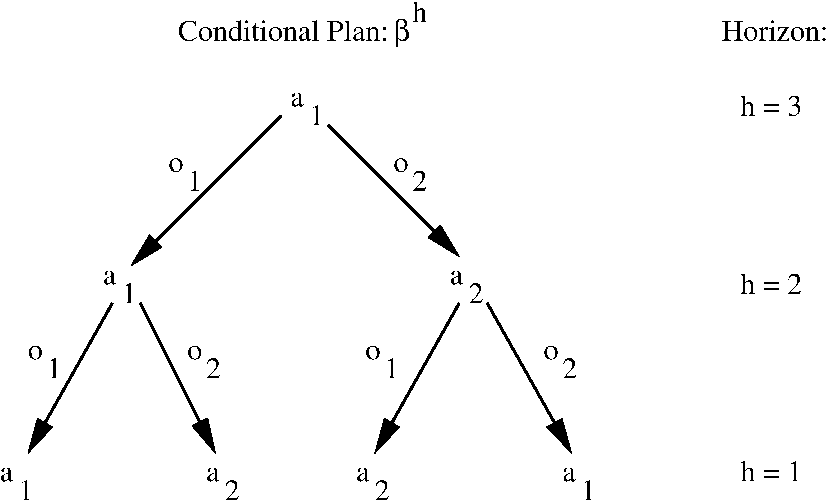
\includegraphics[width=0.4\textwidth]{pics/cond_plan2.pdf}
\hspace{10mm}
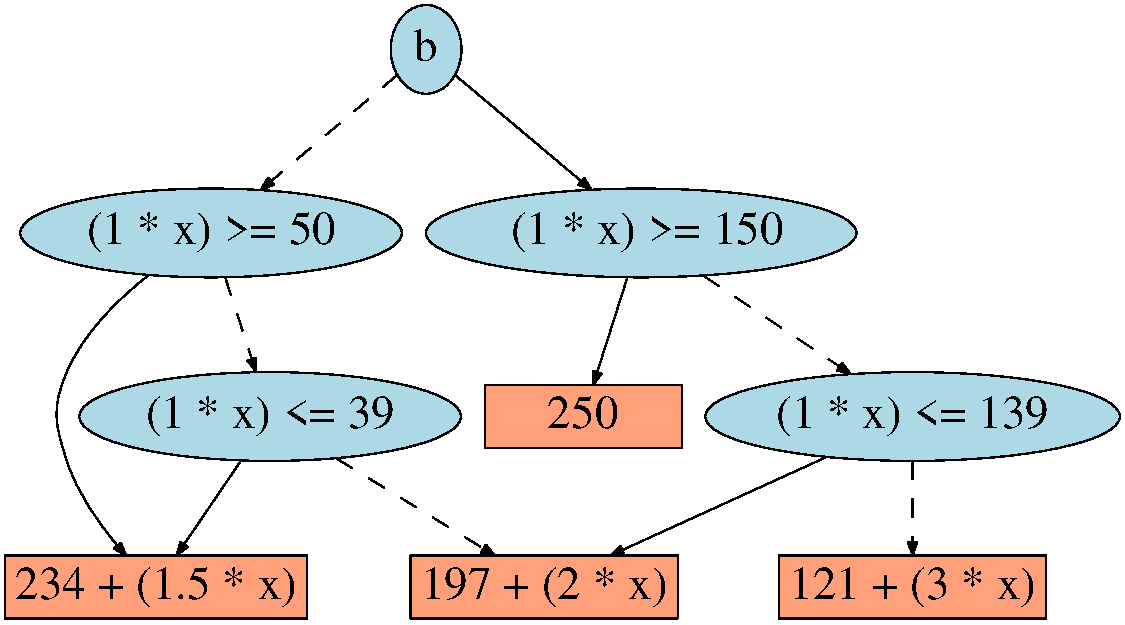
\includegraphics[width=0.45\textwidth]{pics/dag2.pdf}
\end{center}
\vspace{-2mm}
\caption{\footnotesize (left) Example conditional plan $\beta^h$ for
discrete observations; (right) example $\alpha$-function for $\beta^h$
over state $b \in \{0,1\}, x \in \mathbb{R}$ in decision
diagram form: the \emph{true} (1) branch is solid, the \emph{false} (0) branch is
dashed.}
\label{fig:cond_plan}
\end{figure}
%%%%%%%%%%%%%%%%%%%%%%%%%%%%%%%%%%%%%%%%%%%%%%%%%%%%%%%%%%%%%%%%%%%%%%%%
%%%%%%%%%%%%%%%%%%%%%%%%%%%%%%%%%%%%%%%%%%%%%%%%%%%%%%%%%%%%%%%%%%%%%%%%%%%
%\begin{figure}[t]
%\begin{center}
%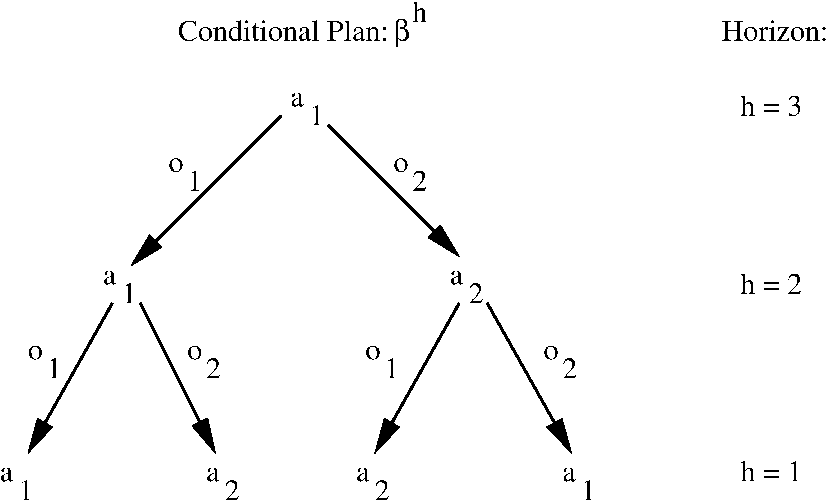
\includegraphics[width=0.4\textwidth]{pics/cond_plan2.pdf}
%\end{center}
%\vspace{-3mm}
%\caption{%\footnotesize 
%The optimal value function for \textsc{\bf Power Plant}
%as a decision diagram: 
%the \emph{true} branch is solid, the \emph{false}
%branch is dashed.} 
%\end{figure}
%%%%%%%%%%%%%%%%%%%%%%%%%%%%%%%%%%%%%%%%%%%%%%%%%%%%%%%%%%%%%%%%%%%%%%%%%%%

\section{Value Iteration for DC-POMDPs}

\label{sec:vi}

In a DC-POMDP, the agent does not directly observe the states and thus
must maintain a belief state $b(\xds) = p(\xds)$.  For a
given belief state $\vec{b} = b(\xds)$, a POMDP policy $\pi$ can be
represented by a tree corresponding to a conditional plan $\beta$.  An
h-step conditional plan $\beta^h$ can be defined recursively in terms
of $(h-1)$-step conditional plans as shown in
Fig.~\ref{fig:cond_plan} (left).
Our goal is to find a policy $\pi$ that maximizes the value function,
defined as the sum of expected discounted rewards over horizon $h$
starting from initial belief state $\vec{b}$:
{\footnotesize
\vspace{-1mm}
\begin{equation}
V^h_\pi(\vec{b}) = E_{\pi} \left[ \sum\nolimits_{t=0}^{h} \gamma^t \cdot r_t \Big| \vec{b}_0 = \vec{b} \right]
\end{equation}
\vspace{-4mm}
}

where $r_t$ is the reward obtained at time $t$ and $\vec{b}_0$ is the
belief state at $t=0$.  For finite $h$ and belief state $\vec{b}$, the
optimal policy $\pi$ is given by an $h$-step conditional plan
$\beta^h$.  For $h = \infty$, the optimal discounted ($\gamma < 1$)
value can be approximated arbitrarily closely by 
a sufficiently large $h$~\cite{kaebling}.  

Even when the state is continuous (but the actions and observations
are discrete), 
the optimal POMDP value function for finite horizon $h$ is a piecewise linear and
convex function of the belief state $\vec{b}$~\cite{Perseus_cont}, hence 
$V^h$ is given by a maximum over a finite set of
``$\alpha$-functions'' $\alpha^h_i$:
{\footnotesize 
\vspace{-1mm}
\begin{equation}
V^h(\vec{b}) = \max_{\alpha^h_i \in \Gamma^h} \l \alpha^h_i, \vec{b} \r = \max_{\alpha^h_i \in \Gamma^h} \int_{\vec{x}_s} \sum_{\vec{d}_s} \alpha^h_i(\xds) \cdot \vec{b}(\xds) \; d\vec{x}_s 
\end{equation}
\vspace{-4mm}
}

Later on when we tackle continuous state \emph{and} observations,
we note that we will dynamically derive an optimal, 
finite partitioning of the observation
space for a given belief state and hence reduce the continuous
observation problem back to a discrete observation problem at every
horizon.  

Given discrete observations $o \in \mathcal{O}^h$, the $\Gamma^h$ in
this optimal $h$-stage-to-go value function can be computed via
Monahan's dynamic programming approach to \emph{value iteration}
(VI)~\cite{monahan82}.  Initializing $\alpha^0_1 = \vec{0}$ and
$\Gamma^0 = \{ \alpha^0_1 \}$, $\Gamma^h$ is obtained from
$\Gamma^{h-1}$ using the backup operation defined in (2):\footnote{The
  $\textrm{\large $\boxplus$}$ of sets is defined as $\textrm{\large
    $\boxplus$}_{j \in \{ 1,\ldots, n \} } S_j = S_1 \textrm{\large
    $\boxplus$} \cdots \textrm{\large $\boxplus$} S_n$ where the
  pairwise cross-sum $P \textrm{\large $\boxplus$} Q = \{ \vec{p} +
  \vec{q} | \vec{p} \in P, \vec{q} \in Q \}$.}  
{\footnotesize
\vspace{-1mm}
\begin{align} 
g^h_{a,o,j}(\xds) &=  \int_{\vec{x}_{s'}} \sum_{\vec{d_{s'}}} p(o|\xds',a)p(\xds'|\xds,a) \alpha^{h-1}_j(\xds') d\vec{x}_{s'}; \hspace{2mm}  \forall \alpha^{h-1}_{j} \in \Gamma^{h-1} \label{eq:backup} \\
\Gamma^{h}_a   &= R(\xds,a) + \gamma \textrm{\large $\boxplus$}_{o \in \mathcal{O}} \left\{ g^h_{a,o,j}(\xds) \right\}_j  \label{eq:cross_prod}\\ 
\Gamma^h  &= \bigcup_a \Gamma^h_a 
\end{align}
\vspace{-4mm}
}

%%%%%%%%%%%%%%%%%%%%%%%%%%%%%%%%%%%%%%%%%%%%%%%%%%%%%%%%%%%%%%%%%%%%%%%%
\incmargin{.5em}
\linesnumbered
\begin{algorithm}[t!]
\footnotesize
\vspace{-.5mm}
\dontprintsemicolon
\SetKwFunction{backup}{Backup}
\SetKwFunction{genObs}{GenRelObs}
\SetKwFunction{prune}{Prune}
\SetKwFunction{remapWithPrimes}{Prime}
\Begin
{
   $V^0:=0, h:=0, \Gamma_{PBVI}^0 = \{ \alpha_1^0 \} $\;
   \While{$h < H$}
   {
       $h:=h+1, \Gamma^h :=\emptyset, \Gamma_{PBVI}^h :=\emptyset$\;
       \ForEach {$\vec{b}_i \in B$}
       {
       	\ForEach {$a \in A$}
      	 {
			$\Gamma_{a}^h :=\emptyset$ \;       		
       		\If {(continuous observations: $q > 0$)}
       			{\emph{// Derive relevant observation partitions $O_i^h$ for belief $\vec{b}_i$} \;
			  $\l O_i^h,p(O_i^h|\vec{b}_i,a) \r \,:=\,$ \genObs{$\Gamma_{PBVI}^{h-1},a,\vec{b}_i$}\;}
       		 \ForEach {$o \in \mathcal{O}_i^{h}$}
       		 {
				\ForEach {$\alpha_j^{h-1} \in \Gamma_{PBVI}^{h-1}$}
       			{
   	 		  		$\alpha_j^{h-1} :=\,$ \remapWithPrimes{$\alpha_j^{h-1}$} 
   	 		  		\emph{// $\forall d_i$: $d_i \to d_i'$ and $\forall x_i$: $x_i \to x_i'$} \; 
%   	 		    	$\Gamma_{a,xd_{o_i},j}^h \,:=\, p(o|xd_{s}) \cdot$ \backup{$\alpha_j^{h},a$}\;
   	 		    	{$g_{a,o,j}^h \,:=\, $ see Eq~\eqref{eq:backup}}
       	      	}
%       	      	$\Gamma_{a,\xdo}^h\,:=\,\textrm{\large $\boxplus$} \Gamma_{a,xd_{o_i}}^h$\;
%       	      	$\Gamma_{a,\xdo}^h\,:=\, $ see Eq~\eqref{eq:cross_prod}\;
       	     }
%           $\Gamma_a^{h} \,:=\,R_a \oplus \gamma \cdot \Gamma_{a,\xdo}^h$\;
            $\Gamma_a^{h} \,:=\, $ see Eq~\eqref{eq:cross_prod}\;
            $\Gamma^{h} \,:=\, \Gamma^{h} \cup \Gamma_a^{h}$\;
       	 }
        	%monahan's pruning first generates all vectors, then prunes
                %but not for PBVI since we only retain alpha-functions provably dominant at a belief point
%              $\Gamma^h \,:=\, $\prune{$\Gamma^h$} \emph{// optional strict dominance testing of $\alpha$-functions}\; 
      }
             % $V^h \,:=\, \mathrm{max}_{\alpha_j \in \Gamma^h} \vec{b}_i \cdot \alpha_j$\;
             % $\pi^{*,h} \,:=\, \argmax_{a} \, \Gamma_a^{h}$\;
      \ForEach {$\vec{b}_i \in B$}
      {
     	$\alpha_{\vec{b}_i}^h :=\ \argmax_{\alpha_j \in \Gamma^h} \alpha_j \cdot \vec{b}_i$\;
     	$\Gamma_{PBVI}^h :=\ \Gamma_{PBVI}^h \cup \alpha_{\vec{b}_i}^h$\;
      }

       \If{$\Gamma_{PBVI}^h = \Gamma_{PBVI}^{h-1}$}
           {break $\,$ \emph{// Terminate if early convergence}\;}
   }
     \Return{$\Gamma_{PBVI}$} \;
}
\caption{\footnotesize \texttt{PBVI}(DC-POMDP, $H$, $B=\left\{\vec{b}_i \right\}$) $\longrightarrow$ $\l V^h \r$ \label{alg:vi}}
\vspace{-1mm}
\end{algorithm}
\decmargin{.5em}
%%%%%%%%%%%%%%%%%%%%%%%%%%%%%%%%%%%%%%%%%%%%%%%%%%%%%%%%%%%%%%%%%

\textbf{Point-based value iteration (PBVI)} computes the value function only for a set of belief states $\{ \vec{b}_i \}$ where $\vec{b}_i := p(\xds)$.  The idea is straightforward and the main modification needed to Monahan's algorithm in Algorithm~\ref{alg:vi} is the loop from lines 19--21 where only $\alpha$-vectors optimal at some belief state are retained for subsequent iterations.  We note that \emph{if} all beliefs reachable in $h$ steps from some initial set can be finitely enumerated and PBVI is executed for this set of beliefs, then optimality is guaranteed for the PBVI policy over these initial beliefs up to horizon $h$.  

%In actuality in the DC-POMDP setting, the generation of continuous observations will most often lead to an infinite number of reachable belief states even in one step, so this optimality guarantee of PBVI will only hold for DC-POMDPs in very special cases when the set of reachable beliefs is finite.  Nonetheless, PBVI has been quite successful in practice without exhaustive enumeration of all reachable beliefs~\cite{pbvi_jair06,hsvi2,Perseus,gapmin}, which motivates our use of PBVI in this work.

We pause for a moment to make a few notes about the \texttt{PBVI}
algorithm in the context of DC-POMDPs.  If we have no continuous
observations ($q=0$), the the discrete observation set is
$\mathcal{O}^h = \{ \vec{d}_o \}, \forall h$ with $p(\vec{d}_o)$ as
defined by~\eqref{eq:obs_model}.  However, if we have continuous
observation variables ($q > 0$) then we will need to derive a relevant
set of observations on line 10, as described in
Section~\ref{sec:cont_obs}.  


\section{Symbolic Dynamic Programming} 

In this section we take a symbolic dynamic programming (SDP) approach
to implementing VI and PBVI as defined in the last section.  To do this,
we need only show that all required operations can be computed efficiently
and in closed-form, which we do next, building on SDP for 
MDPs~\cite{sanner_uai11}.  

\subsection{Case Representation and Extended ADDs}
\label{sec:case}

% operations, max, restrict, substitute
%overview + example plant
The previous \textsc{\bf Power Plant} examples represented all functions in case form,
generally defined as {\footnotesize
\vspace{-1mm}
\begin{align}
f = 
\begin{cases}
  \phi_1: & f_1 \\ 
 \vdots&\vdots\\ 
  \phi_k: & f_k \\ 
\end{cases} \nonumber
\end{align}
\vspace{-4mm}
}

and this is the form we use to represent all functions in a DC-POMDP.
The $\phi_i$ are disjoint logical formulae defined over $\xds$ and/or $\xdo$ with logical ($\land,\lor,\neg$) combinations of boolean variables and inequalities ($\geq,>,\leq,<$) over continuous variables.  
For discrete observation DC-POMDPs, the $f_i$ and inequalities may use any function (e.g., $\sin(x_1) > \log(x_2)\cdot x_3)$; for continuous observations, they are restricted to linear inequalities and linear or piecewise constant $f_i$ as described in Section~\ref{sec:model}.

For \emph{unary operations} such as scalar multiplication $c\cdot f$ (for some constant $c \in \mathbb{R}$) or negation $-f$ on case statements is simply to apply the operation on each case partition $f_i$ ($1 \leq i \leq k$). 
A \emph{binary operation} on two case statements, takes the cross-product of the logical partitions of each case statement and performs the corresponding operation on the resulting paired partitions.  The cross-sum $\oplus$ of two cases is defined as the following:
{\footnotesize 
\vspace{-4mm}
\begin{center}
\begin{tabular}{r c c c l}
&
\hspace{-6mm} 
  $\begin{cases}
    \phi_1: & f_1 \\ 
    \phi_2: & f_2 \\ 
  \end{cases}$
$\oplus$
&
\hspace{-4mm}
  $\begin{cases}
    \psi_1: & g_1 \\ 
    \psi_2: & g_2 \\ 
  \end{cases}$
&
\hspace{-2mm} 
$ = $
&
\hspace{-2mm}
  $\begin{cases}
  \phi_1 \wedge \psi_1: & f_1 + g_1 \\ 
  \phi_1 \wedge \psi_2: & f_1 + g_2 \\ 
  \phi_2 \wedge \psi_1: & f_2 + g_1 \\ 
  \phi_2 \wedge \psi_2: & f_2 + g_2 \\ 
  \end{cases}$
\end{tabular}
\end{center}
\vspace{-2mm}
}
Likewise $\ominus$ and $\otimes$ are defined by subtracting or multiplying partition values.  Inconsistent partitions can be discarded when they are irrelevant to the function value.
A \emph{symbolic case maximization} is defined as below:
\vspace{-4mm}
{\footnotesize
\vspace{-2mm}
\begin{center}
\begin{tabular}{r c c c l}
&
\hspace{-7mm} $\mathrm{max} \Bigg(
  \begin{cases}
    \phi_1: \hspace{-2mm} & \hspace{-2mm} f_1 \\ 
    \phi_2: \hspace{-2mm} & \hspace{-2mm} f_2 \\ 
  \end{cases}$
$,$
&
\hspace{-4mm}
  $\begin{cases}
    \psi_1: \hspace{-2mm} & \hspace{-2mm} g_1 \\ 
    \psi_2: \hspace{-2mm} & \hspace{-2mm} g_2 \\ 
  \end{cases} \Bigg)$
&
\hspace{-4mm} 
$ = $
&
\hspace{-4mm}
  $\begin{cases}
  \phi_1 \wedge \psi_1 \wedge f_1 > g_1    : & \hspace{-2mm} f_1 \\ 
  \phi_1 \wedge \psi_1 \wedge f_1 \leq g_1 : & \hspace{-2mm} g_1 \\ 
  \phi_1 \wedge \psi_2 \wedge f_1 > g_2    : & \hspace{-2mm}f_1 \\ 
  \phi_1 \wedge \psi_2 \wedge f_1 \leq g_2 : & \hspace{-2mm} g_2 \\ 
  \vdots & \vdots
%  \phi_2 \wedge \psi_1 \wedge f_2 > g_1    : & \hspace{-2mm} f_2 \\ 
%  \phi_2 \wedge \psi_1 \wedge f_2 \leq g_1 : & \hspace{-2mm} g_1 \\ 
%  \phi_2 \wedge \psi_2 \wedge f_2 > g_2    : & \hspace{-2mm} f_2 \\ 
%  \phi_2 \wedge \psi_2 \wedge f_2 \leq g_2 : & \hspace{-2mm} g_2 \\ 
  \end{cases}$
\end{tabular}
\end{center}
\vspace{-3mm}
}

The following SDP operations on case statements require more detail than can be provided here, hence we refer the reader to the relevant literature:
%\begin{itemize}
%\item 
{\it Restriction $f|_{\phi}$:}  Takes a function $f$ to restrict only in cases
that satisfy some formula $\phi$ as defined in \cite{sanner_uai11}.
%\item 
{\it Substitution $f\sigma$:} Takes a set $\sigma$ of variables and their substitutions (which may be case statements), and carries out all variable substitutions in sequence~\cite{sanner_uai11}.
%\item 
{\it Integration $\int_{x_1} f dx_1$:}  There are two forms: If $x_1$ is involved in a $\delta$-function (cf. the transition in Eq~\eqref{eq:trans}) then the integral is equivalent to a symbolic substitution and can be applied to any case statement~\cite{sanner_uai11}. Otherwise, if $f$ is restricted to linear constraints and constant values, then the approach of~\cite{sanner_aaai12} can be applied to yield a linearly constained piecewise linear result.
%\end{itemize}

%\vspace{-2mm}
%\emph{Restriction} takes a function $f$ to restrict only in cases
%that satisfy some formula $\phi$, which we write as $f|_{\phi}$.  
%This can be done by simply appending $\phi$ to each case partition
%as the left side shows:
%{\footnotesize
%\begin{center}
%\begin{tabular}{r c c l}
%%&
%%\hspace{-6mm} 
%%  $f = \begin{cases}
%%    \phi_1: & f_1 \\ 
%%   \vdots&\vdots\\ 
%%    \phi_k: & f_k \\ 
%%  \end{cases}$
%%&
%&
%\hspace{0mm}
%  $f|_{\phi} = \begin{cases}
%    \phi_1 \land \phi : & f_1 \\ 
%   \vdots&\vdots\\ 
%    \phi_k \land \phi : & f_k \\ 
%  \end{cases}$
%&
%\hspace{15mm}
%$\int_{x_j'} p(x_j'|\cdots) V'^{h} dx_j' = \begin{cases}
%    \phi_1: & V'^{h} \{ x_j' = f_1 \} \\ 
%   \vdots&\vdots\\ 
%    \phi_k: & V'^{h} \{ x_j' = f_k \}  \\ 
%  \end{cases}$
%  \end{tabular}
%\end{center}
%}
%\emph{Symbolic substitution} simply takes a set $\sigma$ of variables and their substitutions, where
%the LHS of the substitution operator $/$ represents the substitution variable and the
%RHS of the $/$ represents the expression that should be substituted in its place.
%Hence to perform a continuous regression on a more general
%representation, we obtain the right side of the above. 

%xadd representation
The data structure of the \emph{extended algebraic decision diagram}
(XADD)~\cite{sanner_uai11} is used to support case statements and the
required operations.  Figure~\ref{fig:cond_plan} (right) 
is an example of an XADD representation.

%%%%%%%%%%%%%%%%%%%%%%%%%%%%%%%%%%%%%%%%%%%%%%%%%%%%%%%%%%%%%%%%%
%\incmargin{.5em}
%\linesnumbered
%\begin{algorithm}[t!]
%\vspace{-.5mm}
%\dontprintsemicolon
%\Begin{
%	\emph{any function f has $i$ partitions like $\phi_i:f_i$}\;	
%	\emph{compute UB and LB from $\phi_i$ using constraints on $var$}\;
%    $I=$ \emph{ any $var$-independent $\phi_i$} \;
%    $F = $ \emph{differentiate $f_i$}\;
%    $F = I \otimes [F(UB) - F(LB)]$\;
%    \Return{$F$} \;
%}
%\caption{\footnotesize \texttt{VE}($var,f$) $\longrightarrow$ $F$ }
%\vspace{-1mm}
%\end{algorithm}
%\decmargin{.5em}
%%%%%%%%%%%%%%%%%%%%%%%%%%%%%%%%%%%%%%%%%%%%%%%%%%%%%%%%%%%%%%%%%
\subsection{VI for DC State and Discrete Observations} 
\label{sec:disc_obs}

For DC-POMDPs with only discrete observations $o
\in \mathcal{O}$ and observation function $p(o|\xds',a)$ (e.g., 
Eq~\eqref{eq:ex_disc_obs}), we introduce a symbolic version of
Monahan's VI algorithm.  In brief, we note that all VI operations
needed in Section~\ref{sec:vi} apply \emph{directly} to 
DC-POMDPs, e.g., we can rewrite
Eq~\eqref{eq:backup}: {\footnotesize
\vspace{-1mm}
\begin{equation}
g^h_{a,o,j}(\xds) \! =  \!\! \int_{\vec{x}_{s'}} \!\! \bigoplus_{\vec{d_{s'}}} \! \left[ p(o|\xds',\!a) \! \otimes \!\! \left( \! \bigotimes_{i=1}^n p(d_{s_i}'|\xds,\!a) \!\! \right) \!\! \otimes \!\! \left( \! \bigotimes_{j=1}^m p(x_{s_j}'|\xds, \vec{d}_s',\!a) \!\! \right) \!\! \otimes \! \alpha^{h-1}_j(\xds') \! \right] \!\! d\vec{x}_{s'} \label{eq:backup_sdp}
\end{equation}
\vspace{-4mm}
}

Crucially we note since the continuous transition cpfs $p(x_{s_j}'|\xds, \vec{d}_s',a)$ are deterministic and hence defined with Dirac $\delta$'s (e.g., Eq~\ref{eq:trans}) as described in Section~\ref{sec:model}, the integral $\int_{\vec{x}_{s'}}\!$ can always be computed in closed case form as discussed in Section~\ref{sec:case}.
In short, nothing additional is required for PBVI on DC-POMDPs
in this case --- the key insight
is simply that $\alpha$-functions are now represented by
case statements and can ``grow'' with the horizon as they partition the
state space more and more finely.
%%%%%%%%%%%%%%%%%%%%%%%%%%%%%%%%%%%%%%%%%%%%%%%%%%%%%%%%%%%%%%%%%
\incmargin{.5em}
\linesnumbered
\begin{algorithm}[t!]
\footnotesize 
\vspace{-.5mm}
\dontprintsemicolon
\SetKwFunction{substitute}{Substitute}

\Begin
{
		\For {$\alpha_j(\xdsp) \in \Gamma^{h-1}$}    
		{
		\emph{// Point-based backup (PBB) operation}\\
    	$\alpha_j(\xds,\xdo) := \int_{\vec{x}_s'} \bigoplus_{\vec{d}_s'} p(\xdo|\xdsp,a) \otimes p(\xdsp| \xds,a) \otimes \alpha_j(\xdsp) \; d\vec{x}_s'$\;
		}  
		\ForEach {$\alpha_j(\xds,\xdo)$}    
		{
		\emph{// Generate value of $\alpha$-vector for belief $\vec{b}_i(\xds)$ as a function of observations}\\
		$\delta_{j}(\xdo) := \int_{\vec{x}_{s}} \bigoplus_{\vec{d}_s} \vec{b}_i(\xds) \otimes \alpha_j(\xds,\xdo) \; d\vec{x}_s$\\ \;
		}
		\emph{// Generate observation partitions -- see text for details}\\
		$\mathcal{O}^h := \max(\delta_1(\xdo),\ldots,\delta_{j}(\xdo))$\;

	\ForEach {$o_k \in \mathcal{O}^h$}{
    	  \emph{// Let $\phi_{o_k}$ be the partition constraints for observation $o_k \in \mathcal{O}^h$}\\
            $p(\mathcal{O}^h = o_k|\vec{b}_i) := \int_{x_s'} \int_{x_o} \int_{x_s} \bigoplus_{d_o} \bigoplus_{d_s} \bigoplus_{d_s'} p(\xdo|\xds',a) \otimes p(\xds'|\xds,a) \otimes \vec{b}_i \otimes  \mathbb{I}[\phi_{o_k}] d_{x_o} d_{x_s}d_{x_s'}$ \;
        }
    \Return{$\l \mathcal{O}^h, p(\mathcal{O}^h|\vec{b}_i,a) \r$} \;
    %do this for each belief in B
}
\caption{\footnotesize \texttt{GenRelObs}($\Gamma^h,a,\vec{b}_i$) $\longrightarrow$ $\l \mathcal{O}^h, p(\mathcal{O}^h|\vec{b}_i,a) \r$ }
\label{alg:genrelobs}
\vspace{-1mm}
\end{algorithm}
\decmargin{.5em}
%%%%%%%%%%%%%%%%%%%%%%%%%%%%%%%%%%%%%%%%%%%%%%%%%%%%%%%%%%%%%%%%%
\subsection{PBVI for DC State and DC Observations} 
\label{sec:cont_obs}

In general, it would be impossible to apply standard VI to 
DC-POMDPs with continuous observations since the number of observations
is infinite.  However, building on ideas in~\cite{pascal_ijcai05},
in the case of PBVI, it is possible to \emph{derive} a finite set of
continuous observation partitions that permit exact point-based backups.
This additional operation (\texttt{GenRelObs}) appears on line 10 of PBVI in 
Algorithm~\ref{alg:vi} in the case of continuous observations and is
formally defined in Algorithm~\ref{alg:genrelobs}.

To demonstrate the generation of relevant continuous observation partitions, 
we use the second iteration of the \textsc{\bf Cont. Obs. 1D-Power
  Plant} along with two beliefs points represented as 
uniform distributions: $b_1: U(t_s;2,6)$ and $b_2: U(t_s;6,11)$ as
shown in Figure~\ref{fig:beliefs} (left).

Starting with an empty set of
relevant observation partitions $\mathcal{O}^h$, the algorithm first
eliminates the next state variable $\xds'$. It regresses the
the set of
$\alpha$-vectors of the previous horizon back one step via
the transition and observation model: $\alpha_j(\xds,\xdo) :=
\int_{x_s'} \bigoplus_{x_d'} p(xd_{o_i}|xd'_{s_i},a)  \otimes  p(xd'_{s_i}| xd_{s_i},a) \otimes  \alpha_j\hspace{1mm}dx_s'
$.  This operation of line 5 in \texttt{GenRelObs} is similar to 
the point-based backup in~\eqref{eq:backup}. For
continuous variables the continuous integral and for discrete
variables the restriction operation is used as defined in
Section~\ref{sec:case}.  
Assuming that after $h=1$ the set of $\alpha$-vectors are
defined equal to the reward function of equation (1).
%{\footnotesize
%\vspace{-3mm}
%\begin{align}
%\alpha_1^1(t_s) &= 
%\begin{cases}
% (t_s>200) &: -1000 \\
%\neg(t_s>200) &: 100 \\
%\end{cases}
%\hspace{10mm} 
%\alpha_2^1(t_s) = \top: -1 \nonumber
%\end{align}
%}
For $h=2$ the resulting $\alpha$-vectors after the regression step are functions of the observation and current state: 
{\footnotesize
\vspace{-2mm}
\begin{align}
\alpha_{close}^2(t_s,t_o) &= 
\begin{cases}
 (t_s<15)\wedge (t_s - 10 < t_o<t_s) &: 10 \\
(t_s>15)\wedge (t_s - 10 < t_o<t_s) &: -100  \\
\neg(t_s - 10 < t_o<t_s) &: 0
\end{cases}
\hspace{2mm} 
\alpha_{open}^2(t_s,t_o) &= \begin{cases}
(t_s - 10 < t_o<t_s) &: -0.1 \\
\neg(t_s - 10 < t_o<t_s) &: 0
\end{cases}
\nonumber
\end{align}
} 
We now need the $\alpha$-vectors as a function of the observation
space for a particular belief state, thus next we eliminate the
current state variable in line 6--8. The resulting $\delta$-functions
now only depend on the observation: $\delta_{j}^{\vec{b}_i}(\xdo) := $
$\int_{x_s'} \bigoplus_{x_d'} \vec{b}_i  \otimes  \alpha_j(\xds,\xdo) \hspace{1mm}dx_s'$.  For $b_2: U[t_s;6,11]$
%assume the following simple $\delta$-functions:
the resulting $\delta$-functions are defined below:
{\footnotesize
%\vspace{-2mm}
\begin{align}
\delta_{close}^{b_2}(t_o) &= 
\begin{cases}
 (14 < t_o< 18) &: 0.025*t_o - 0.45\\
 (8 < t_o< 14) &:  - 0.1\\
 (4 < t_o< 8) &: - 0.025*t_o -0.1\\
\end{cases}
\hspace{5mm} 
\delta_{open}^{b_2}(t_o) &= \begin{cases}
 (15 < t_o< 18) &: 25*t_o - 450\\
 (14 < t_o< 15) &: - 2.5*t_o - 37.5\\
 (8 < t_o< 14) &:  -72.5\\
 (5 < t_o< 8) &: - 25*t_o + 127.5\\
 (4 < t_o< 5) &:  2.5*t_o - 10\\
\end{cases}
\nonumber
\end{align}
%\vspace{-5mm}
}
%{\footnotesize
%\begin{align}
%\delta_{1}(t_o) &= 
%\begin{cases}
% (2<t_o<6) &: 15 - 2.5*t_o \\
%(-4<t_o<2) &: 10 \\
%(-8<t_o<-4) &: 20 + 2.5*t_o 
%\end{cases}
%\hspace{5mm} 
%\delta_{2}(t_o) &= \begin{cases}
% (2<t_o<6) &: -0.15 + 0.025*t_o \\
%(-4<t_o<2) &: -0.1 \\
%(-8<t_o<-4) &: -0.2 - 0.025*t_o 
%\end{cases}
%\nonumber
%\end{align}
%}
%%%%%%%%%%%%%%%%%%%%%%%%%%%%%%%%%%%%%%%%%%%%%%%%%%%%%%%%%%%%%%%%%%%%%%%%%%
\begin{figure*}[tbp!]
\vspace{-3mm}
\centering
\hspace{-20mm}
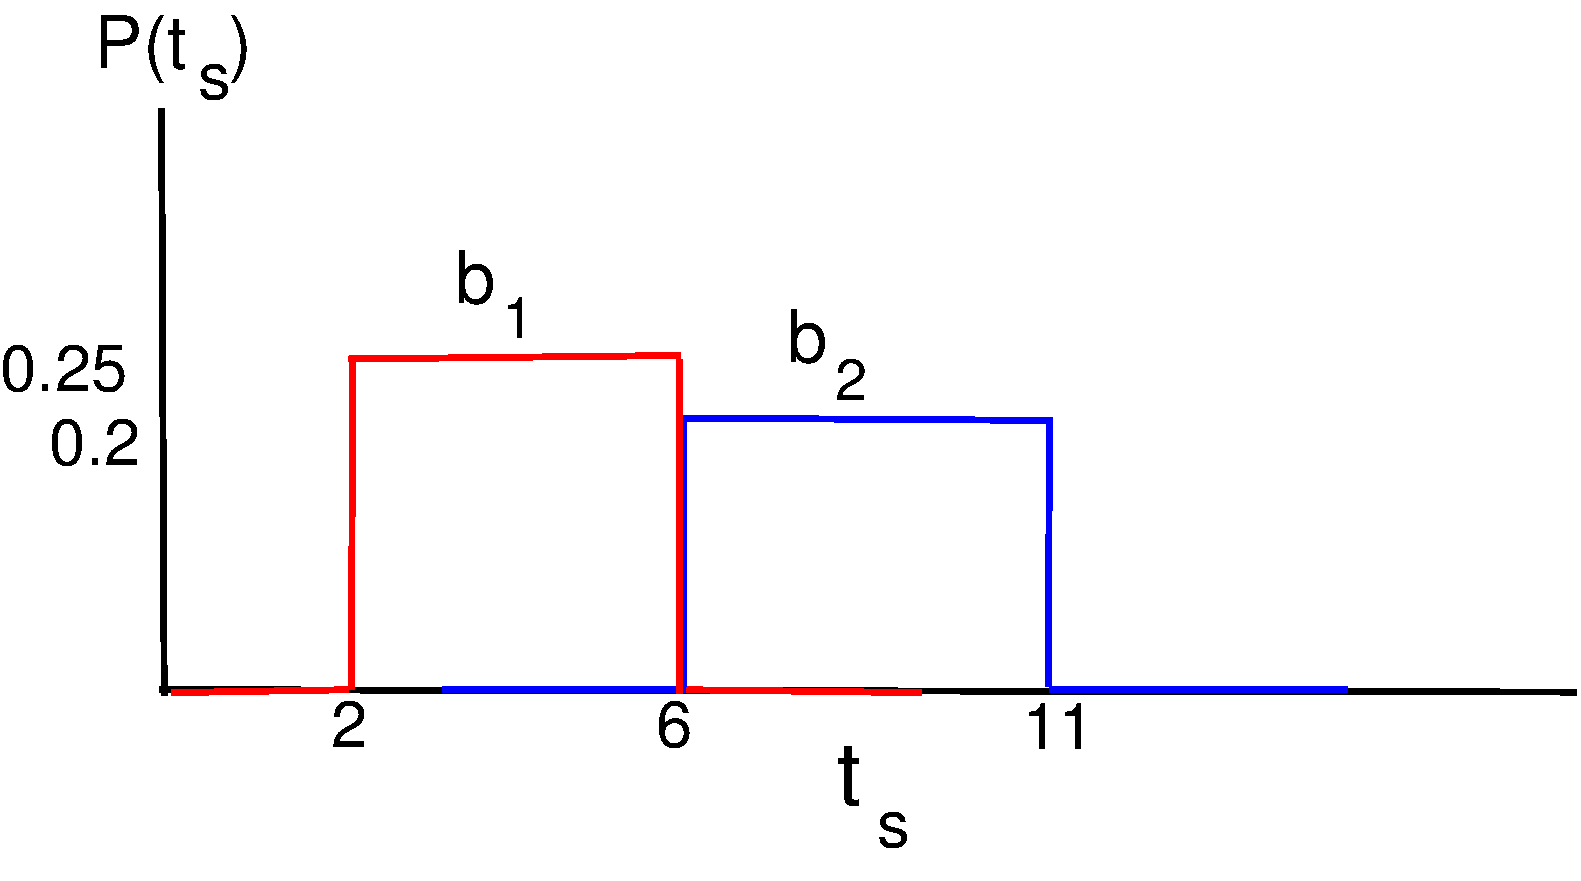
\includegraphics[width=0.42\textwidth]{pics/beliefs_2.pdf}
\hspace{10mm}
%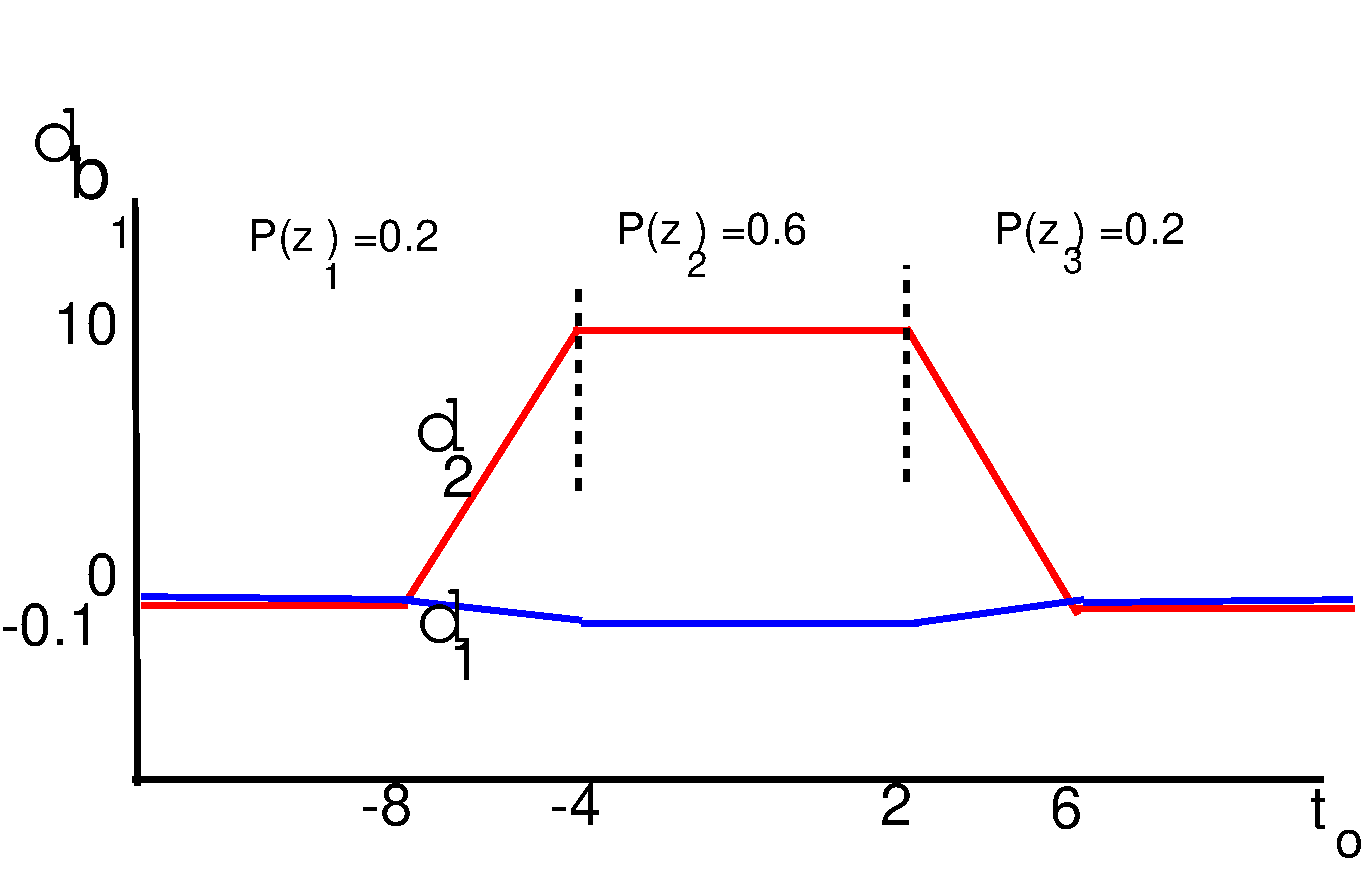
\includegraphics[width=0.33\textwidth]{pics/delta_b1.pdf}
%\hspace{-2mm}
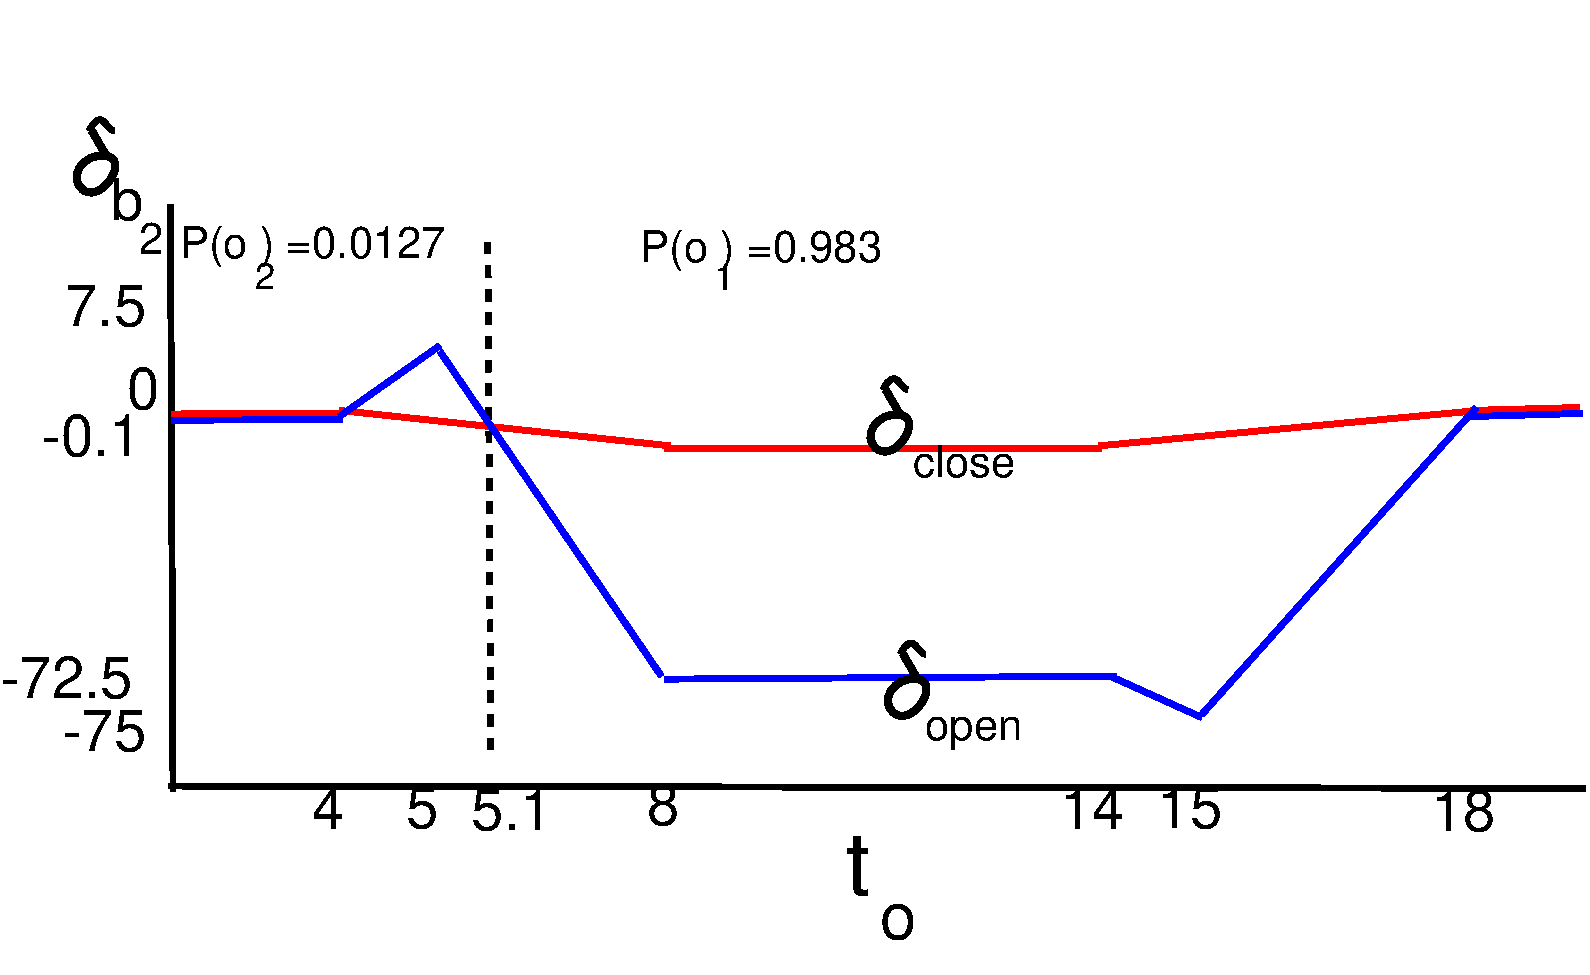
\includegraphics[width=0.42\textwidth]{pics/delta_b2_2.pdf}
\hspace{-17mm}
\vspace{-2mm}
\caption{\footnotesize 
{\it (left)} Beliefs $b_1,b_2$ for 1D \textsc{\bf Power Plant} example; 
%{\it (center)} Observation dependent function for $b_2$ that partition the observation space into 5 regions with different probabilities for $p(o_1),p(o_2)$ ; 
{\it (right)} Relevant observation partitions and their probabilities for $b_2$. This diagrams shows that for temperatures $t_o < 5.1$ the policy is to open the valve and for higher temperatures, it is unsafe to open it and the policy should follow $\delta_{close}(t_o)$ which is to close the valve. 
}
\label{fig:beliefs}
%\vspace{-4mm}
\end{figure*}
%%%%%%%%%%%%%%%%%%%%%%%%%%%%%%%%%%%%%%%%%%%%%%%%%%%%%%%%%%%%%%%%%%%%%%%%%% 
The observation dependent $\delta$-functions divide the observation space into regions which can yield the optimal policy according to the belief state $b_2$. According to continuous observation space defined in \cite{pascal_ijcai05}, for a 1-dimensional observation space with two or more functions of the observation, we need to find the optimal boundaries or partitions of the space. In their work, numerical solutions are proposed to find the roots of any two observation dependent function. Instead, here we leverage the symbolic power of the max-operator defined in Section~\ref{sec:case} to find all the boundary regions that define for what partitionings of the observation each 
$\delta$-function is optimal. For the two $\delta$-functions above the following partitions of the observation space is derived after taking their maximum in lines 9--11: 
{\footnotesize
\vspace{-2mm}
\begin{align}
\mathrm{max} \Bigg(\delta_{close}^{b_2}(t_o),\delta_{open}^{b_2}(t_o)\Bigg) &= 
\begin{cases}
o_1: (14 < t_o< 18) &: 0.025*t_o - 0.45\\
o_1: (8 < t_o< 14) &:  -0.1\\
o_1: (5.1 < t_o< 8) &: - 0.025*t_o -0.1\\
o_2: (5 < t_o< 5.1) &: - 25*t_o + 127.5\\
o_2: (4 < t_o< 5) &:  2.5*t_o - 10\\
\end{cases}
\nonumber
\end{align}
}
Note here that each partitioned is labeled according to the original $\delta$-function where $o_1$ is the label of the partition coming from $\delta_{close}^{b_2}(t_o)$. 
These partitions define observation regions which we can now use in a similar fashion to a discrete observation set if only the probability of each of the two distinct observation partitions is found.  This is demonstrated visually
in Figure~\ref{fig:beliefs} (right) for $b_2$. %Note here that the maximum of the $\delta$-functions for $b_2$ is equal to $\delta_{open}^{b_2}(t_o)$.

Now with the observation partitions derived, all that remains is to
calculate probabilities for these relevant observations conditioned on
the belief state. 
% This does not check out!
% 
%As a reality check, we note that if we integrate out the
%state and observation from the observation model and the belief state
%regardless of a particular $\alpha$-vector, it integrates to one:
%$\int_{\xdo}\int_{\xds} p(\xdo|\xds',a)*p(\xds'|\xds,a)*p(s) = 1$.
Thus we only need to multiply the indicators of each observation partition 
in this formula to obtain the probability mass lying in each
partition:
$$p(o_k|\vec{b}_i) := \int_{x_s'}\int_{x_o}\int_{x_s} \bigoplus_{d_o} \bigoplus_{d_s} \bigoplus_{d_s'} p(\xdo|\xds',a)*p(\xds'|\xds,a)*\vec{b}_i* \mathbb{I}[\phi_{o_k}] d_{x_o} d_{x_s}d_{x_s'}$$
For our example the non-zero probabilities occur in the following partitions as below:
{\footnotesize
\vspace{-2mm}
\begin{align}
p(o_k|b_2) &= 
\begin{cases}
(\phi_1 : 14 < t_o< 18) & : 0.2\\
(\phi_2 : 8 < t_o< 14) & :  0.6\\
(\phi_3 : 5.1 < t_o< 8) & : 0.183\\
(\phi_4 : 5 < t_o< 5.1) & : 0.0002\\
(\phi_5 : 4 < t_o< 5) & :  0.0125\\
\end{cases}
\nonumber
\end{align}
}
where each constraint is defined as $\phi_i$. For any number of actions and observations the total number of observation partitions depends on the number of belief points. In our example we must have two observation probabilities which is defined as the sum of the probabilities for $o_1,o_2$ according to the constraints: 
\begin{align*}
o_1&: \phi_1 \vee \phi_2 \vee \phi_3 \longrightarrow p(o_1|b_2)=0.983 \\
o_2&: \phi_4 \vee \phi_5  \longrightarrow p(o_2|b_2)=0.0127
\end{align*}
%{\footnotesize
%\begin{align}
%p(z_k)=
%\begin{cases}
% (t_o<2) &: 0.2 \\
%(2<t_o) &: 0.8\\
%\end{cases} 
%\nonumber
%\end{align}
%}

Hence we can now use the algorithms and methods of a discrete observation setting using the probabilities of the partitioned observation space in PBVI! 
We note here that our method applies to a restricted class of piecewise functions which is piecewise linear transitions and piecewise constant reward and belief. The main reason is that the integration operation over continuous states and observations only allows constant or linear constraints (upper or lower bounds) over these variables \cite{sanner_aaai12}. Thus although in theory we can apply this approach to any piecewise polynomial function, in practice it is limited by the integration bounds.  %Figure ~\ref{fig:obsPartition} shows the observation partitions obtained in the 1D problem instance for different horizons and their related probabilities. In a lyx file, needed?
Next we present some results for 2-dimensional continuous observation spaces.

%%%%%%%%%%%%%%%%%%%%%%%%%%%%%%%%%%%%%%%%%%%%%%%%%%%%%%%%%%%%%%%%%%%%%%%%%%
%\begin{figure}[tbp!]
%\vspace{-2mm}
%\centering
%\includegraphics[width=0.42\textwidth]{pics/nodes.pdf}\\
%\vspace{-2mm}
%\includegraphics[width=0.42\textwidth]{pics/time.pdf}
%\vspace{-2mm}
%\caption{\footnotesize space 
%and time vs. horizon.
%}
%\label{fig:timeSpace}
%\vspace{-4mm}
%\end{figure}
%%%%%%%%%%%%%%%%%%%%%%%%%%%%%%%%%%%%%%%%%%%%%%%%%%%%%%%%%%%%%%%%%%%%%%%%%%

\section{Empirical Results}
We evaluated our continuous POMDP solution using XADDs on the
\textsc{\bf 1D-Power Plant} example and another variant of this
problem with two variables, described below.\footnote{ Full problem
specifications and Java code to reproduce these experiments are available online in
Google Code: \textit{http://code.google.com/p/cpomdp} .}

%%%%%%%%%%%%%%%%%%%%%%%%%%%%%%%%%%%%%%%%%%%%%%%%%%%%%%%%%%%%%%%%%%%%%%%%%%
\begin{figure*}[tbp!]
\vspace{2mm}
\centering
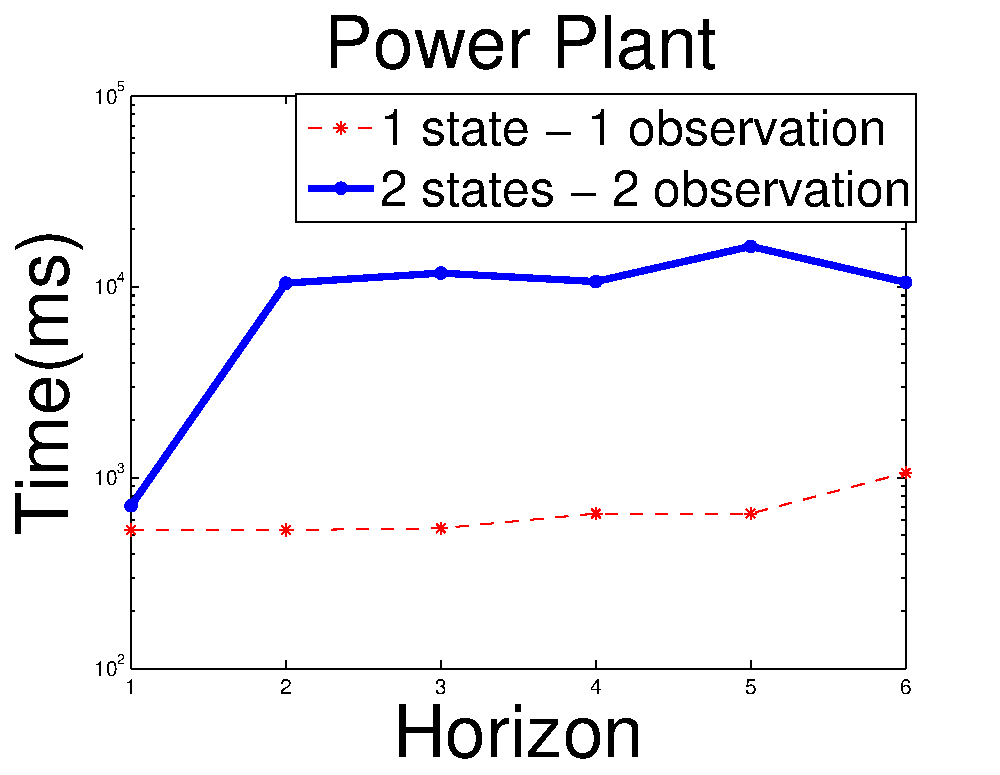
\includegraphics[width=0.32\textwidth]{pics/time2.pdf}
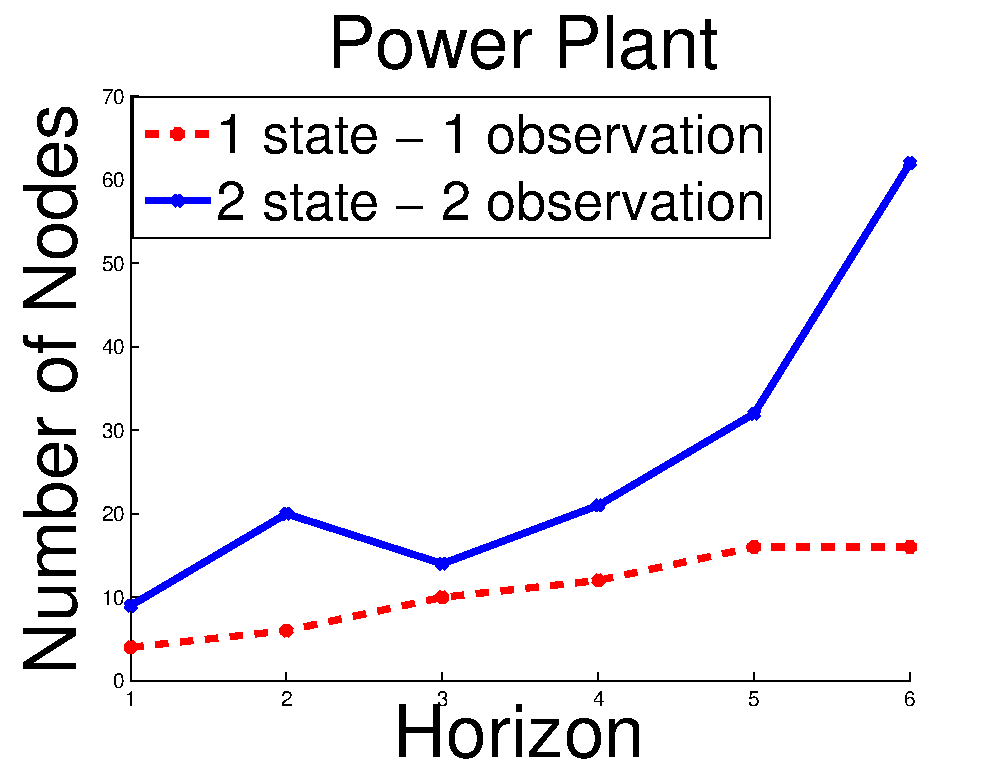
\includegraphics[width=0.32\textwidth]{pics/nodes2.pdf}
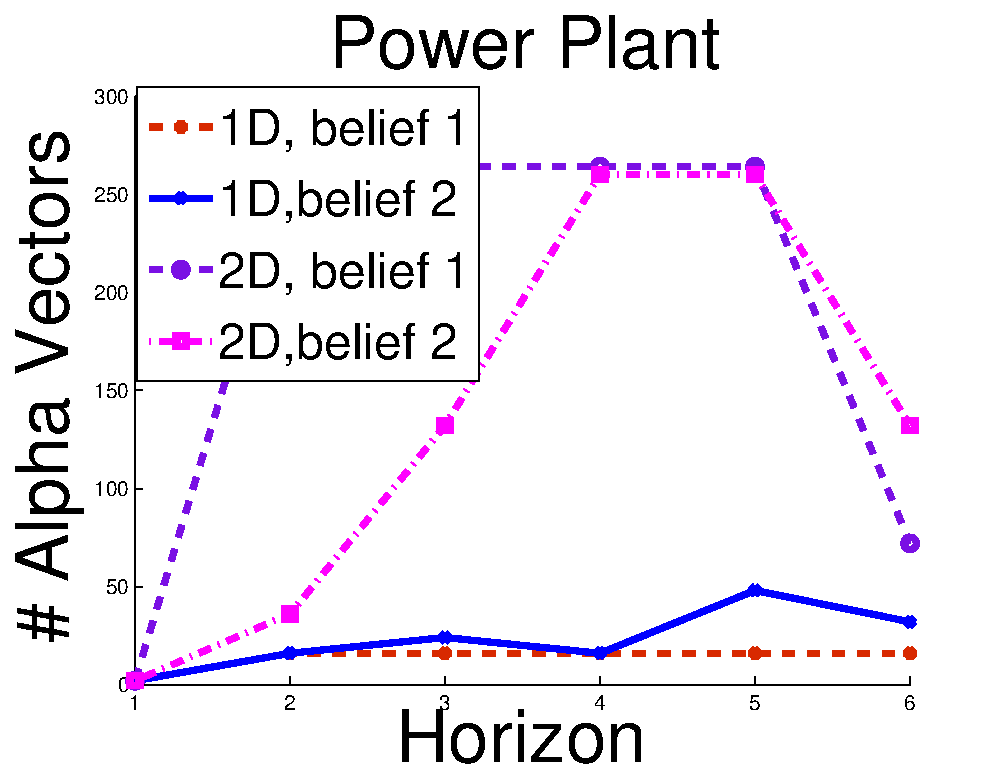
\includegraphics[width=0.32\textwidth]{pics/alpha-vectors2.pdf}
\vspace{-1mm}
\caption{\footnotesize 
{\it (left)} Space vs Horizon; 
{\it (center)} Time vs Horizon; 
{\it (right)} Number of $\alpha$-vectors vs Horizon.
}
\label{fig:timeSpace}
%\vspace{-4mm}
\end{figure*}
%%%%%%%%%%%%%%%%%%%%%%%%%%%%%%%%%%%%%%%%%%%%%%%%%%%%%%%%%%%%%%%%%%%%%%%%%% 

{\bf \textsc{\bf 2D-Power Plant}:} We consider the more complex model of the power plant similar to \cite{steam2} where the pressure inside the water tank must be controlled to avoid mixing water into the steam or explosion of the tank. We model the pressure variable $p$ as a partially observable variable from the observation readings of the pressure $po$. The two actions of increase and decrease are defined based on the change in both the temperature and the pressure. For the increase action we define: %the transition functions and the reward function is defined as below: 
{\footnotesize
\begin{align}
p(p_s'|\vec{p_s},inc)&= \delta\left[ p_s' - 
\begin{cases}
 (p+10> 20) &: 20 \\ 
\neg (p+10> 20) &: p_s + 10 \\
\end{cases}
\right]\nonumber
\hspace{5mm} 
p(t_s'|\vec{t_s},inc)= \delta\left[ t_s' - (t_s +10) \right]\nonumber
\end{align}
}
There is a high reward for staying withing the safe temperature and pressure range since it produces power, else depending on how safe it is to have values higher or lower than the safe range, penalty is defined.
{\footnotesize
\vspace{-3mm}
\begin{align}
R(t_s,p_s,inc) &= 
\begin{cases}
(5 \leq p_s \leq 15)\wedge (95 \leq t_s \leq 105)&:50\\
(5 \leq p_s \leq 15)\wedge (t_s \leq 95)&: -1\\
%(5 \leq p_s \leq 15)\wedge (t_s \geq 95)&: -3\\				
%(p_s \leq 5) &: -3\\						
(p_s \geq 15) &: -5\\ 
else &: -3
\end{cases}\nonumber
\end{align}
}
As for the decrease action, the transition functions reduce the temperature by 5 units and the pressure by 10 units as long as the pressure stays above zero. For the reward function, we assume that there is always a small penalty for decreasing the values because power can not be generated. 
For the observation model we consider two continuous uniform distributions such as the following:  
{\footnotesize
\begin{align}
p(t_o|t_s') = 
\begin{cases}
(t_s + 80<t_o<t_s+ 105) &: 0.4 \\
 \neg (t_s + 80<t_o<t_s+ 105) &: 0 \\
\end{cases}\nonumber
\hspace{5mm} 
p(p_o|p_s') = 
\begin{cases}
(p_s<p_o<p_s+10) &: 0.1 \\
 \neg(p_s<p_o<p_s+10) &: 0 \\
\end{cases}\nonumber
\end{align}
}
We define two rectangular uniform beliefs around the regions of rewarding, so that one needs to increase the values while the other should decrease them: $b_1: U[t_s;90,100]*U[p_s;0,10]$ and $b_2: U[t_s;90,130]*U[p_s;10,30]$
%\begin{align}
%b_1 = 
%\begin{cases}
%(p_o>p_s) \wedge (p_o<p_s+10) \wedge (t_o>t_s+ 90) \wedge (t_o<t_s+ 100)&: 0.01 \\
% \neg( (p_o>p_s) \wedge (p_o<p_s+10) \wedge (t_o>t_s+ 90) \wedge (t_o<t_s+ 100)) &: 0 \\
%\end{cases}\nonumber
%\end{align}
%\begin{align}
%b_2 = 
%\begin{cases}
%(p_o>p_s +10) \wedge (p_o<p_s+30) \wedge (t_o>t_s+ 90) \wedge (t_o<t_s+ 130)&: 0.00125 \\
% \neg((p_o>p_s +10) \wedge (p_o<p_s+30) \wedge (t_o>t_s+ 90) \wedge (t_o<t_s+ 130)) &: 0 
%\end{cases}\nonumber
%\end{align}
% I can draw this and the 1D belief
In Figure ~\ref{fig:timeSpace}, a time and space analysis of
the two versions of \textsc{\bf Power Plant} have been performed for up to 6 horizons. %Comparing the two problem sizes demonstrates the effect of the number of state-observation variables in our algorithm. 
As the algorithm progresses, the time required to compute the probability of the partitions and finding the maximum $\alpha$-vector with respect to beliefs increases for both problem sizes and significantly more for the 2D version. %The stability in time is due to the fact that each stage almost takes the same time since it has converged quickly.%???
Increase in the problem size, increases the partition numbers on the observation space and this produces more $\alpha$-vectors which also effects the space required to perform the algorithm. The number of vectors stays the same for most horizons and they drop after convergence in the 2D problem instance. %The number of nodes in each iteration increases as more space is required to perform higher iterations.
This shows that although the 2D instance takes more time and space than the 1D instance, it still converges within reasonable resources.

In Figure ~\ref{fig:3D}  we present plots of the maximum $\delta$-vectors of belief $b_1$ for different iterations of the 2D problem instance. %Each plot demonstrates the value of each vector as a function of the pressure and temperature. 
Starting with the first iteration, the value is highest for the reward range ($5<p<15 \wedge 95<t<105$) and -1 or less for other places. In the fifth iteration, the value function has partitioned into more pieces, showing how higher temperatures can increase the value without considering the effect of the pressure. In the last plot, horizon $h=6$ has better tuned the value function so that higher temperatures and pressures increase the value of the maximum $\delta$-vector and also within the reward range, finer grain partitions have been formed. %Also note that the policy depends on the initial belief and for these plots they were based on $b_1$ which was lower than the reward range. The first action would then mean it has performed an increase while the other iterations decrease and increase respectively.  
%%%%%%%%%%%%%%%%%%%%%%%%%%%%%%%%%%%%%%%%%%%%%%%%%%%%%%%%%%%%%%%%%%%%%%%%%%
% policy2, v2plot.pdf, v9plot
% annotation?
\begin{figure*}[tbp!]
%\vspace{-2mm}
\centering
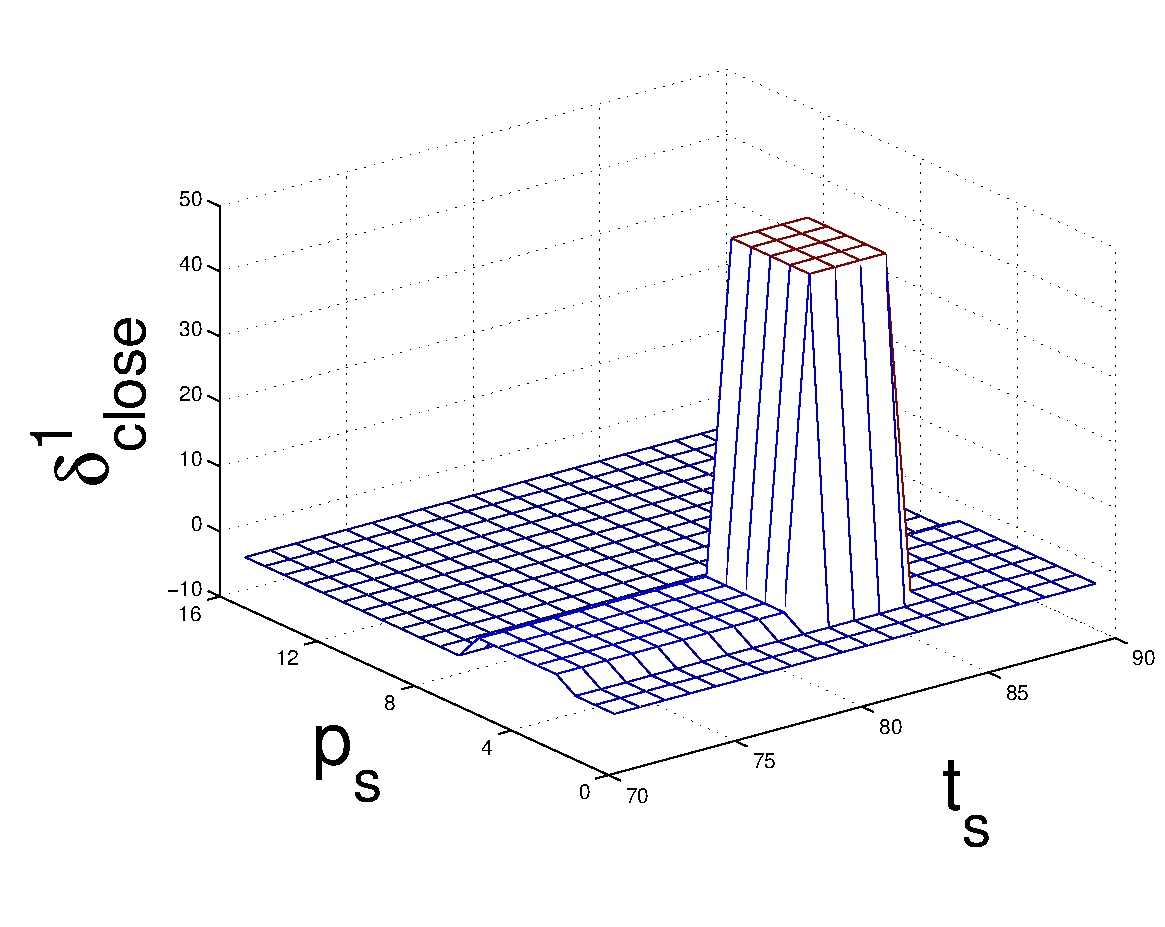
\includegraphics[width=0.31\textwidth]{pics/2d1-4.pdf}
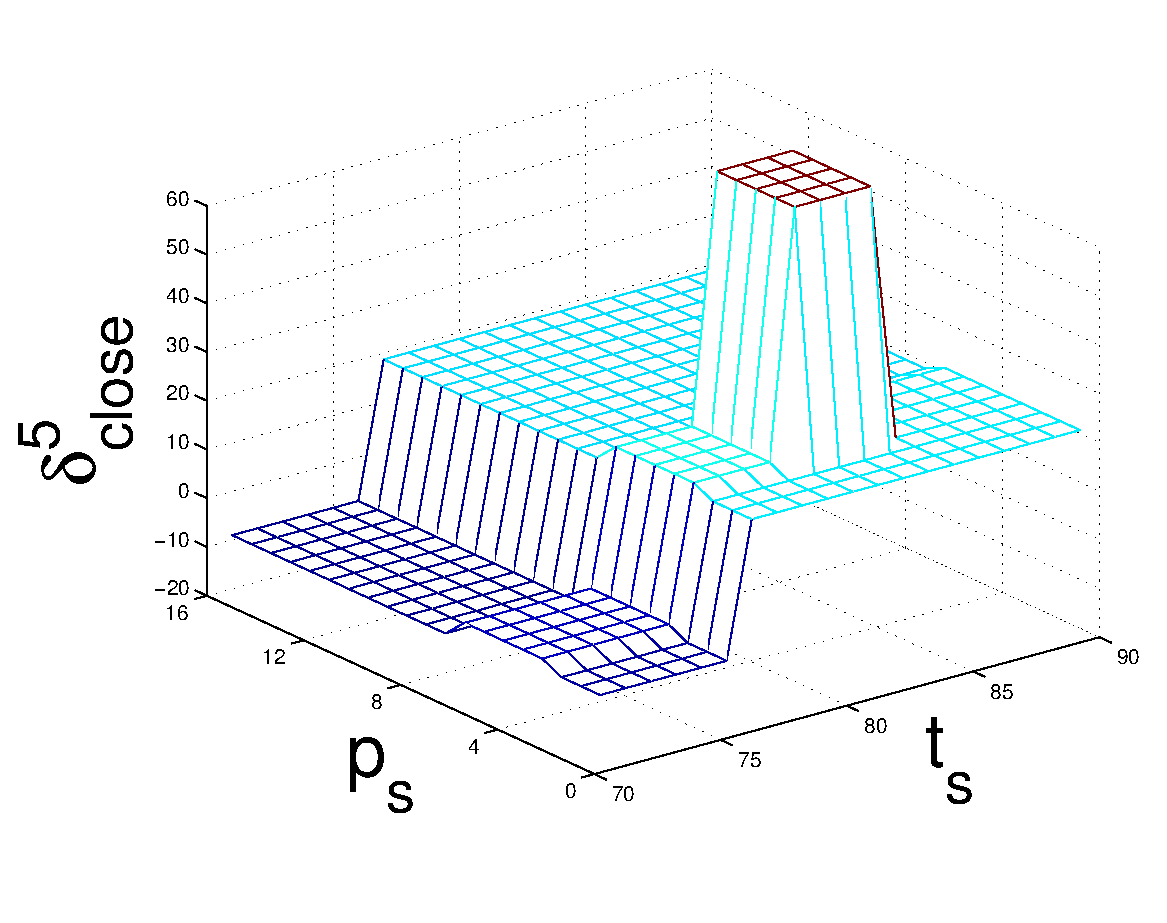
\includegraphics[width=0.31\textwidth]{pics/2d9-4.pdf}
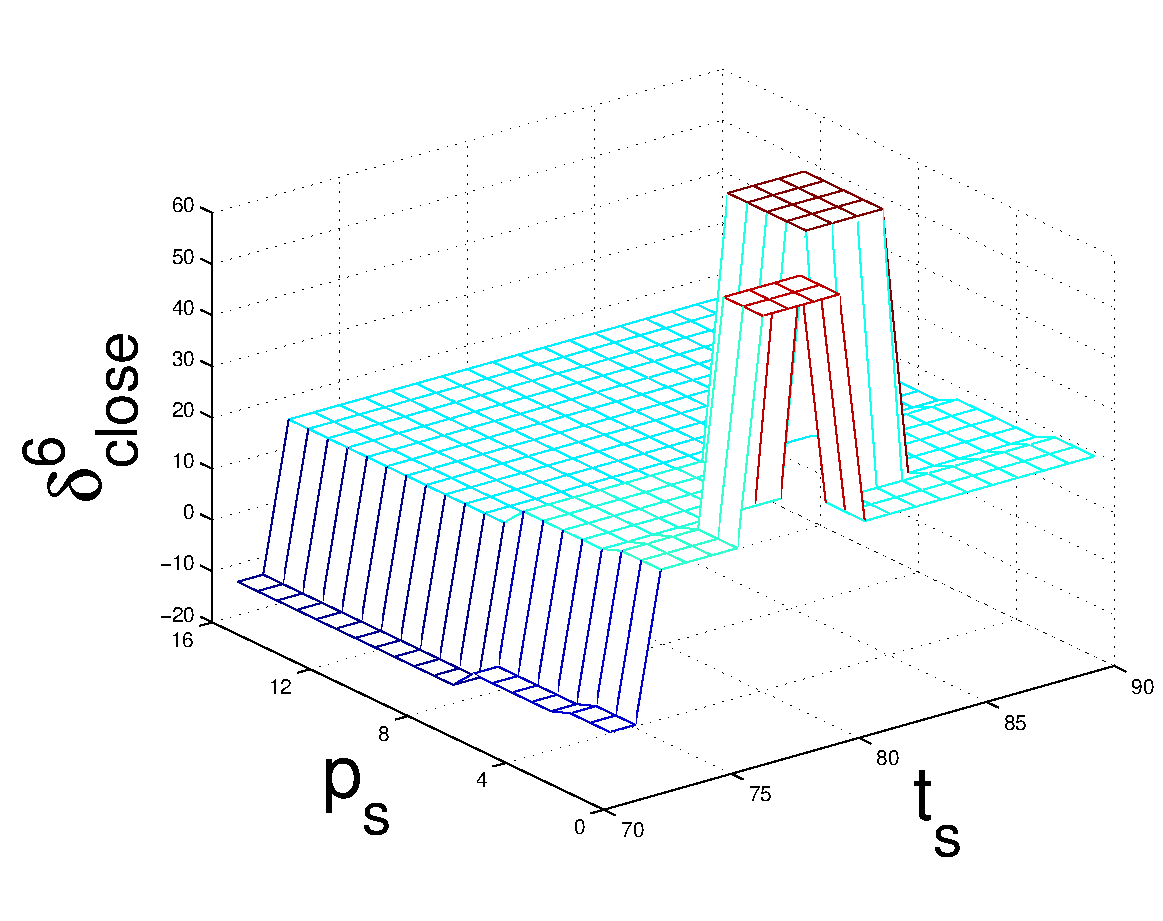
\includegraphics[width=0.31\textwidth]{pics/2d111-4.pdf}
\vspace{-3mm}
\caption{\footnotesize 
{\it (left)}Maximum $\delta$-vector for $b_1$ and action of $close$ in first iteration; 
{\it (center)} $\delta_{close}^5(b_1)$; 
{\it (right)} $\delta_{close}^6(b_1)$. Finer grain partitions show that closing (or opening) the valve can occur at more exact temperatures at higher horizons. 
}
\label{fig:3D}
%\vspace{-4mm}
\end{figure*}
%%%%%%%%%%%%%%%%%%%%%%%%%%%%%%%%%%%%%%%%%%%%%%%%%%%%%%%%%%%%%%%%%%%%%%%%%% 

\section{Conclusion} 
%This work has used the concept of continuous states and the SDP solution to MDPs from ~\cite{sanner_uai11} and continuous observations from the work of \cite{pascal_ijcai05}. It is exclusive in the sense that it brings together the continuous state and observation POMDPs using a symbolic approach. 
%In many applications of the POMDP framework, the state and observation space have been considered as discrete values such as ~\cite{steam2} here we avoid this general simplification and work with the real values from sensors.
%%sampling, monte carlo, particle filter, gaussians, perseus, pergeus
%
%There has been prior work on approximate solutions to POMDPs with large or continuous state spaces ~\cite{Thrun99h}, ~\cite{Perseus} and some has been extended to the continuous observation setting using methods such as sampling ~\cite{Perseus_cont}.
%In most approximate continuous state POMDP work, continuous or large discrete actions has been used. Thus we can extend the current work using \cite{zamani_aaai12} to contain continuous actions and provide exact or approximate solutions. 
%
%%\section{Conclusion}
We presented the first exact symbolic operations for \texttt{PBVI} in
expressive DC-POMDPs with continuous state \emph{and} observations.
Unlike related work that has extended to the continuous state and
observation setting~\cite{Perseus_cont}, we do not approach the
problem by sampling.  Rather, following~\cite{pascal_ijcai05}, the key
contribution of this work was to define a discrete set of observation
partitions on the multivariate continuous observation space via
symbolic maximization techniques and derive the related probabilities
using symbolic integration.  An important avenue for future work is to
determine whether similar techniques can be applied to the difficult
case of continuous state, observation, \emph{and} action DC-POMDPs.

\subsubsection*{Acknowledgments}

NICTA is funded by the Australian Government as represented by the Department of Broadband, Communications and the Digital Economy and the Australian Research Council through the ICT Centre of Excellence program. This work was supported by the Fraunhofer ATTRACT fellowship STREAM and by the EC, FP7-248258-First-MM.
%\subsubsection*{References} 
\bibliography{dcpomdp}
\bibliographystyle{plain}

\end{document}
